\documentclass[a4paper,12pt]{memoir}

% \usepackage{lipsum}
% package for generating dummy text -- remove for actual thesis

\usepackage{amsmath,amssymb,amsthm} % standard AMS LaTeX packages

\usepackage{listings} % for typesetting programming code and similar elements
\lstset{
  columns=flexible,
  basicstyle={\small\ttfamily},
}

\usepackage{pdfpages}
\usepackage{lu-thesis}
% load after amsmath!
% requires the memoir document class as well as the following packages:
% ebgaramond, ebgaramond-maths, graphicx, hyperref, newtxmath, xparse
% load with 'times' option to use a Times New Roman replacement as default font

\usepackage[backend=biber, style=ieee, sorting=nty]{biblatex}
\addbibresource{bibliography.bib}
% bibliography

\usepackage{tikz}     % used for displaying in-document graphics
\usetikzlibrary{shapes}
\usepackage{enumitem} % used to customize enumerate 
\usepackage{subfiles} % used to compile pdfs for sections separately

\usepackage{xcolor} % access to more colours
\definecolor{lundblue}{RGB}{0,0,128}
\definecolor{lundbronze}{RGB}{156,97,20}

\usepackage[colorlinks]{hyperref}
% package for generating hyperlinks
% load after all other packages to avoid compatibility issues (unless a package
% complains and say you should do otherwise)
\hypersetup{%
  colorlinks=true,%
  linkcolor=lundblue,%
  urlcolor=lundblue,%
  citecolor=lundbronze,%
}

%%%% BEGIN example usage of amsthm package

\numberwithin{equation}{section} % preface equation number with section number

% equations, theorems, propositions, lemmas and corollaries share the same counter
\theoremstyle{plain} %\theoremstyle{theorem}

\newtheorem*{utheorem}{Theorem} % unnumbered Theorem environment
\newtheorem{theorem}[equation]{Theorem} 
\newtheorem{proposition}[equation]{Proposition}
\newtheorem{lemma}[equation]{Lemma}
\newtheorem{corollary}[equation]{Corollary}

\theoremstyle{definition} % these environments are not typeset in italics, but
                          % the environment's name is typeset in boldface
\newtheorem*{udefinition}{Definition} % unnumbered Definition environment
\newtheorem{definition}[equation]{Definition}

\theoremstyle{remark} % these environments are not typeset in italics, and
                      % environment's name is typeset in italics instead of boldface
\newtheorem{remark}[equation]{Remark}
\newtheorem{example}[equation]{Example}

%%%% END example usage of amsthm package

\begin{document}

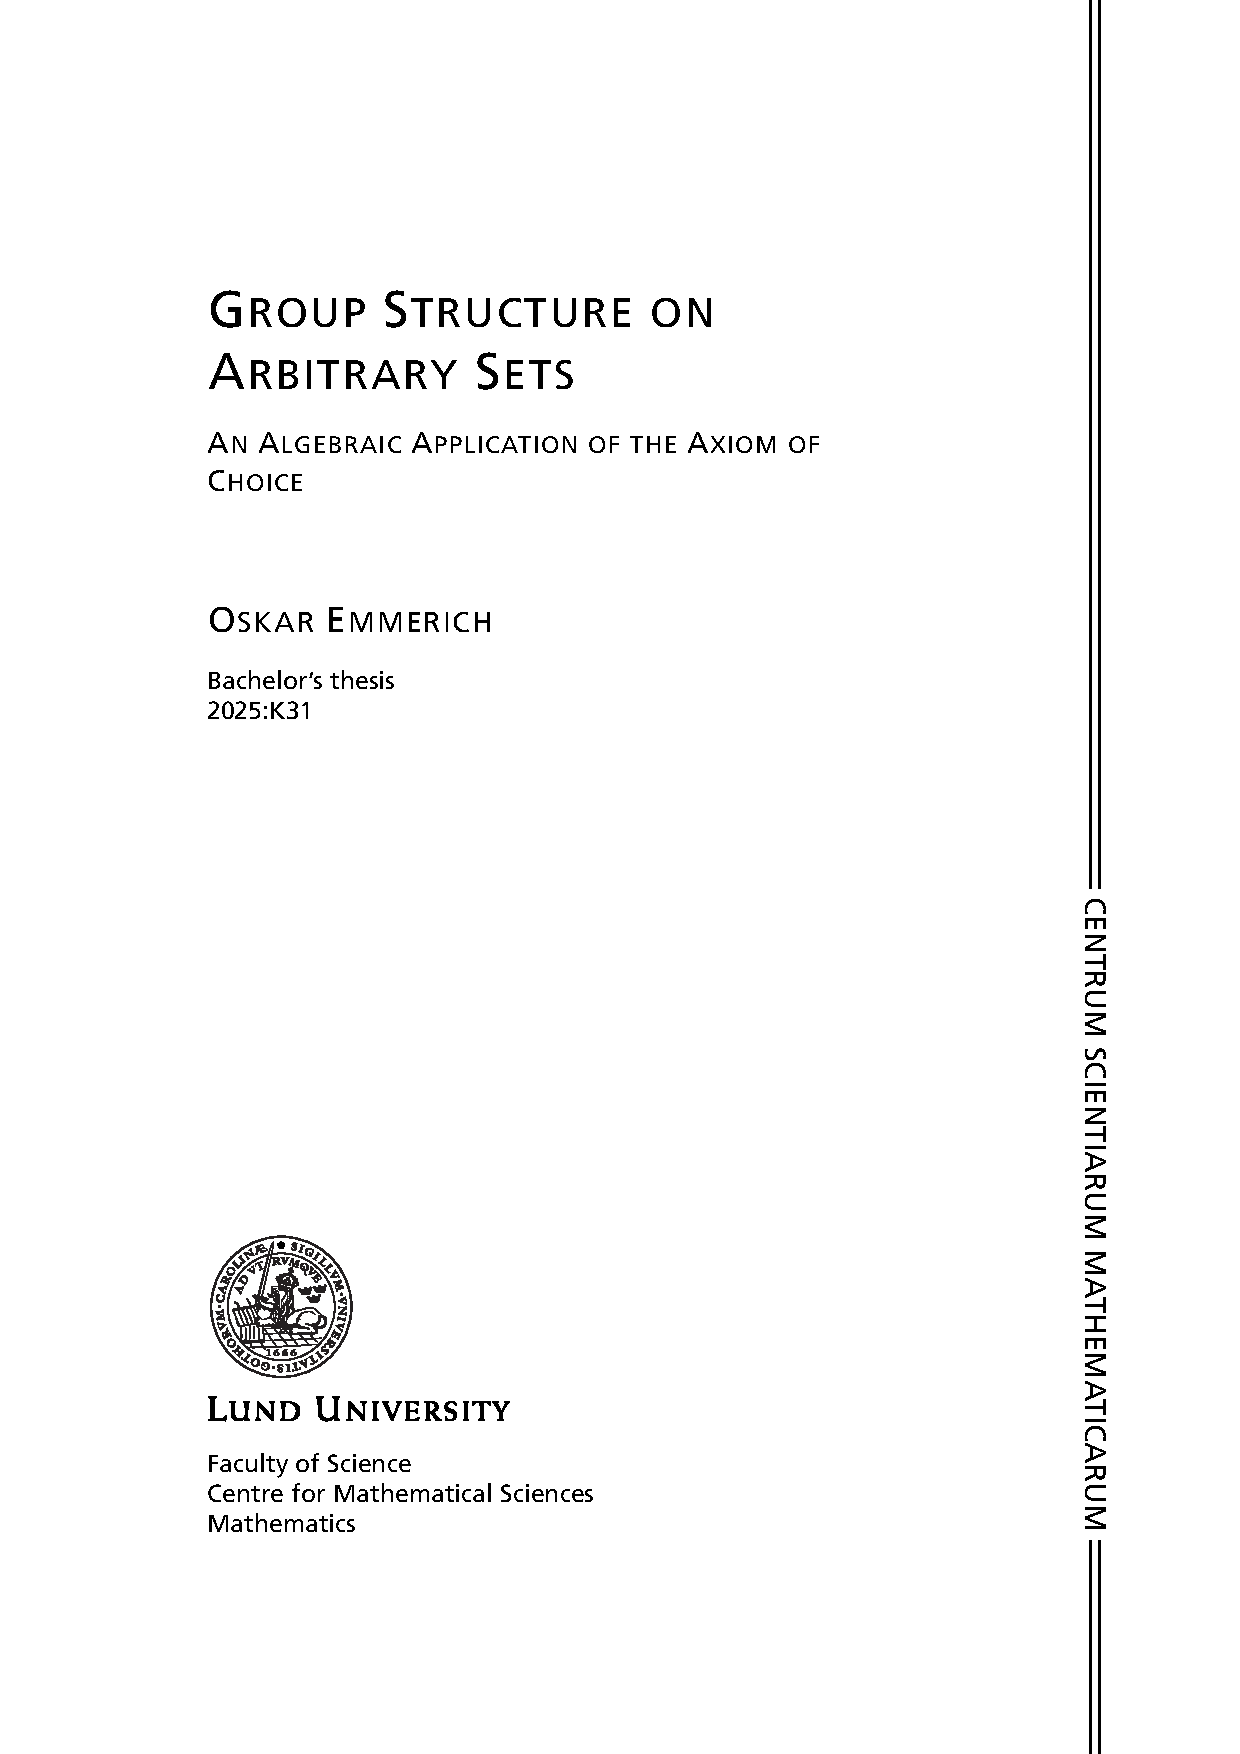
\includepdf[pages={1}]{cover_page_2025.pdf}
\cleardoublepage

%%%%% BEGIN cover page

\author{Oskar Emmerich}
% the thesis' author

\title{Group structure on arbitrary sets:\\An algebraic application of the Axiom of Choice}
% the thesis' title

\date{11th September 2025}
% the thesis' hand-in date

\maketitleLU{Bachelor's}{Anitha Thillaisundaram} % comment for master's thesis
% \maketitleLU[Master's][Advisor's name] % uncomment for master's thesis

%%%%% END cover page

\frontmatter % pages within the front matter are numbered using lowercase Roman numerals

%%%%% BEGIN abstract

\thispagestyle{empty}

\begin{abstract}
  In 1972 Hajnal and Kertész published a paper proving that the Axiom of Choice is equivalent to the assertion that a groupoid structure can be defined on every set.
  This thesis aims to provide the necessary background needed for this proof.
  In the first part basic concepts in set theory such as the Well-Ordering Theorem are derived. 
  This culminates in a lemma by Hartogs (1915) in which it is shown, without the Axiom of Choice, that for every set there exists an ordinal with cardinality greater than that of the set.
  The second part then gives an introduction to model theory with the aim to prove the Löwenheim-Skolem Theorem.
  This theorem states that every theory with an infinite model also has infinite models of any given power.
  The final part of the thesis then examines the proof from Hajnal's and Kertész's paper in detail.
\end{abstract}

%%%%% END Abstract

%%%%% BEGIN popsci description

\chapter*{Acknowledgements}
I would like to thank Anitha Thillaisundaram for being my thesis advisor and for all the helpful suggestions and feedback she provided.

I would like to thank my family as well as my friends both in Lund and in Frankfurt. 
I appreciate the patience and support you gave me during the entire writing process.
I would also like to extend my thanks the regulars of the mathematics student council (MUR) room, where large parts of this thesis were conceptualized and written.
You were there whenever I needed to explain something in order to understand it myself.

Lastly I would like to thank Tomas Persson for taking the time to be my examiner.

\chapter*{Popular Science Description}
\addcontentsline{toc}{chapter}{Popular Science Description}
\subfile{sections/popular_description/popular_description}

%%%%% END popsci description

%%%%% BEGIN toc

\cleardoublepage

\settocdepth{section}
\tableofcontents*

%%%%% END toc

%%%%% BEGIN intro

\chapter*{Introduction}
\addcontentsline{toc}{chapter}{Introduction}
\subfile{sections/introduction/introduction}

%%%%% END intro

%%%%% BEGIN main body of the thesis

\mainmatter % pages within   the main matter are numbered using Arabic numerals

\chapter{Preliminaries}\label{preliminaries}
\subfile{sections/preliminaries/preliminaries}

\chapter{Orderings and Well-Orderings}\label{orderings}
\subfile{sections/well_orderings/well_orderings}

\chapter{Model Theory}\label{model-theory}
\subfile{sections/model_theory/model_theory}

\chapter{Hajnal's and Kertész's Theorem}
\subfile{sections/main_theorem/main_theorem}

%%%%% END main body of the thesis

%%%%% BEGIN appendices

\appendix % appendices are numbered using uppercase Roman letters

%%%%% END appendices

\backmatter

%%%%% BEGIN references

%\bibliographystyle{alpha}
%\bibliography{bibliography}
\printbibliography

%%%%% END references

\includepdf[pages={2}]{cover_page_2025.pdf}

\end{document}